% Standalone pgfplots: SAVANT cell phi vs IIT4 distinction phi (H_624).
% N=20 paired samples across 5 gain profiles x 4 cells; rho=0.86, r=0.97.
% Native LaTeX, no Python dep. `make figures` compiles to figures/fig02_isomorphism_scatter.pdf.
\documentclass[border=4pt]{standalone}
\usepackage{pgfplots}
\pgfplotsset{compat=1.18}
\begin{document}
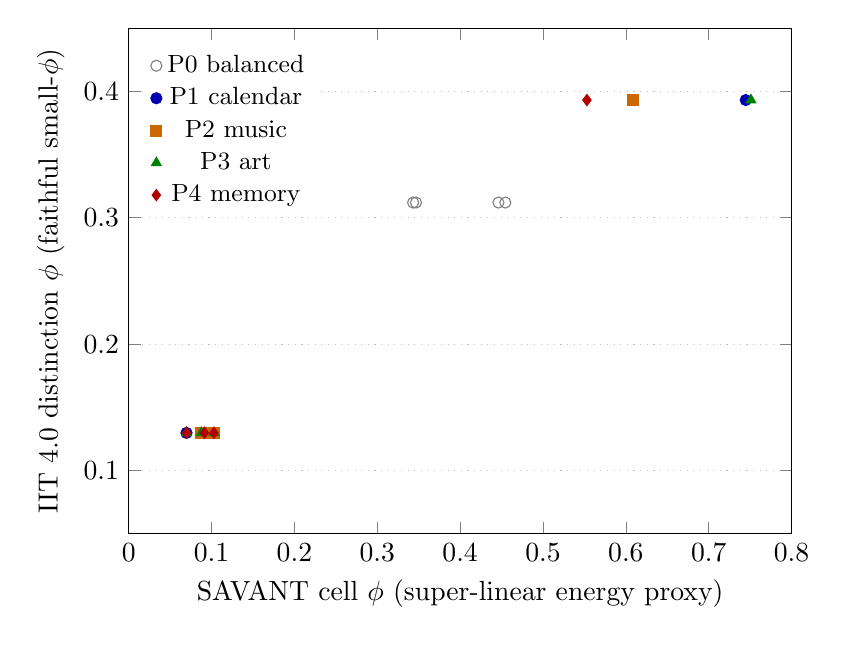
\begin{tikzpicture}
\begin{axis}[
    width=10cm, height=8cm,
    xlabel={SAVANT cell $\phi$ (super-linear energy proxy)},
    ylabel={IIT 4.0 distinction $\phi$ (faithful small-$\phi$)},
    xmin=0, xmax=0.8, ymin=0.05, ymax=0.45,
    legend style={at={(0.02,0.97)}, anchor=north west, draw=none, font=\small},
    ymajorgrids, grid style={dotted},
]
% P0 BALANCED (4-fold tie on dist side)
\addplot[only marks, mark=o, gray] coordinates
  {(0.45455,0.31203) (0.34325,0.31203) (0.44621,0.31203) (0.34667,0.31203)};
% P1 CALENDAR dominant
\addplot[only marks, mark=*, blue!70!black] coordinates
  {(0.74468,0.39314) (0.06975,0.12973) (0.09147,0.12973) (0.08750,0.12973)};
% P2 MUSIC dominant
\addplot[only marks, mark=square*, orange!80!black] coordinates
  {(0.10285,0.12973) (0.60888,0.39314) (0.09147,0.12973) (0.08750,0.12973)};
% P3 ART dominant
\addplot[only marks, mark=triangle*, green!50!black] coordinates
  {(0.10285,0.12973) (0.06975,0.12973) (0.75098,0.39314) (0.08750,0.12973)};
% P4 MEMORY dominant
\addplot[only marks, mark=diamond*, red!70!black] coordinates
  {(0.10285,0.12973) (0.06975,0.12973) (0.09147,0.12973) (0.55302,0.39314)};
\legend{P0 balanced, P1 calendar, P2 music, P3 art, P4 memory}
\end{axis}
\end{tikzpicture}
\end{document}
